\documentclass[journal]{IEEEtran}
\usepackage[utf8]{inputenc}
\usepackage{amsmath}
\usepackage{amsfonts}
\usepackage{amssymb}
\usepackage{graphicx}
\usepackage[left=2cm,right=2cm,top=2cm,bottom=2cm]{geometry}
\usepackage[export]{adjustbox}
\usepackage{subfigure,color,amsmath,amssymb,amsfonts}
\usepackage{url,graphicx,subfigure}

% Some handy Latin commands
\newcommand{\etal}{\textit{et al}.}
\newcommand{\ie}{\textit{i}.\textit{e}.,}
\newcommand{\eg}{\textit{e}.\textit{g}.}

\begin{document}
\title{Modeling a MIMO-OFDM Wireless System}
\author{Alon S. Levin\thanks{The Cooper Union, Department of Electrical Engineering}\\Wireless Communications\\ECE-408 --- Spring 2020}
\maketitle

\begin{abstract}
Three wireless systems are simulated: MIMO, OFDM and a hybrid MIMO-OFDM system. Different equalization techniques, including pre-coding, zero-forcing, and MMSE are implemented and their performances compared across varying SNR levels.
\end{abstract}

\begin{IEEEkeywords}
MIMO, OFDM, pre-coding, zero-forcing, MMSE, IEEE802.11a
\end{IEEEkeywords}

%%%%%%%%%%%%%%%%%%% Introductions %%%%%%%%%%%%%%%%%%
\section{Introduction}\label{sec:intro}
In this project, several different MIMO and OFDM techniques are analyzed individually and in tandem. MIMO (Multi-Input, Multi-Output) systems use multiple transmitters and receivers to increase performance; OFDM (Orthogonal Frequency-Division Multiplexing) is a multi-carrier technique that works to negate the effects of inter-symbol interference (ISI) in wireless channels.

Three MIMO techniques are explored in this project:
\begin{itemize}
\item Pre-Coding,
\item Zero-Forcing, and
\item MMSE.
\end{itemize}
These are described in Sec.~\ref{sec:MIMO}.

Two OFDM techniques are explored in this project:
\begin{itemize}
\item Zero-Forcing, and
\item MMSE.
\end{itemize}
These are described in Sec.~\ref{sec:OFDM}.

Finally, the six possible combinations of these techniques are explored as well. These are described in Sec.~\ref{sec:MIMO-OFDM}.

\section{MIMO} \label{sec:MIMO}
A MIMO link can be represented mathematically as 
\begin{equation}
y = \mathbf{H}x + n,
\end{equation}
wherein $x$ is the vector of transmitted signals, $\mathbf{H}$ is the channel matrix, $n$ is a vector of AWGN noise, and $y$ is the vector of received signals. In this project, a $2\times2$ MIMO link was simulated across three different channels.

\subsection{Pre-Coding}
Channel pre-coding is dependent on knowledge of the channel at both transmitter and receiver. The channel matrix $\mathbf{H}$ can be decomposed at both ends of the link by singular value decomposition (SVD):
\begin{equation}
\mathbf{H} = \mathbf{U \Sigma V}^H,
\end{equation}
in which the matrix $\mathbf{\Sigma}$ is a diagonal matrix of the singular values of $\mathbf{H}$. 

At the transmitter, the signal $x$ is left-multiplied by $\mathbf{V}$; at the receiver, the received signal is left multiplied by $\mathbf{U}^H$. The result, then, is:
\begin{align}
y & = \mathbf{U}^H(\mathbf{HV}x + n) \\
& = \mathbf{U}^H(\mathbf{U \Sigma V}^H \mathbf{V}x + n) \\
& = \mathbf{\Sigma}x + \mathbf{U}^Hn.
\end{align}

Left-multiplying by $\mathbf{\Sigma}^{-1}$ would therefore allow the recovery of the original signal $x$.

\subsection{Zero-Forcing Equalizer}
The zero-forcing equalizer attempts to approximate the inverse of the channel by computing a linear filter to the received signal to correct channel interference. A benefit of this equalizer is that it only requires knowledge of the channel at the receiver.

The zero-forcing equalizer is represented by the following equation:
\begin{equation}
\mathbf{W}_{ZF} = (\mathbf{H}^H \mathbf{H})^{-1}\mathbf{H}^H.
\end{equation}

\subsection{MMSE Equalizer}
A similar equalizer is the MMSE equalizer. It improves on the zero-forcing equalizer by taking into account the noise variance $\sigma^2_n$ present in the channel:
\begin{equation}
\mathbf{W}_{MMSE} = (\mathbf{H}^H \mathbf{H} + \sigma^2_n\mathbf{I})^{-1}\mathbf{H}^H,
\end{equation}
where $\mathbf{I}$ is the identity matrix.

\subsection{Comparison of Results}
A plot of the BER versus SNR is shown in Fig.~\ref{fig:mimo_res}. A QAM $2\times2$ MIMO system was simulated over three random Gaussian flat fading channels; the average results are plotted. Pre-coding and zero-forcing proved to have similar performance; MMSE likewise had similar performance in the presence of high AWGN noise, but  was outperformed under high-SNR conditions.

\begin{figure}[!htbp]
    \centering
    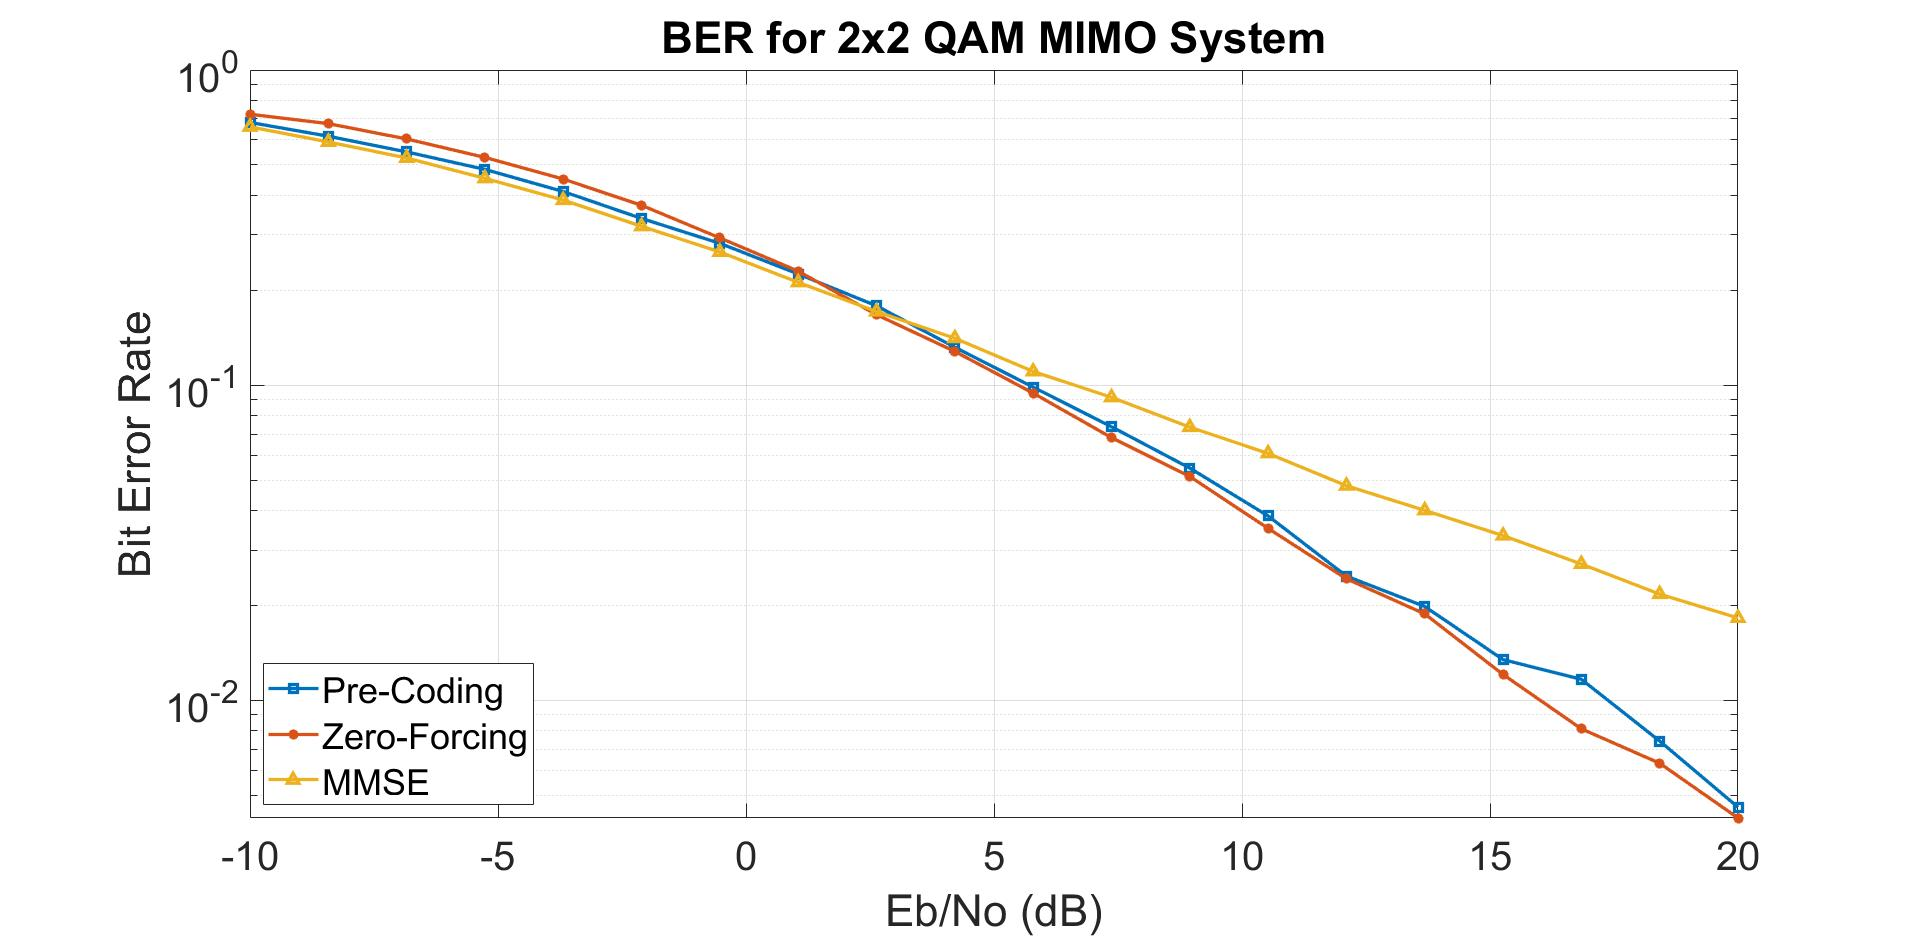
\includegraphics[width = 0.45\textwidth]{MIMO.jpg}
    \caption{BER plot for a $2\times2$ QAM MIMO system using different MIMO algorithms.}
    \label{fig:mimo_res}
\end{figure}

\section{OFDM} \label{sec:OFDM}
OFDM seeks to transmit a signal over multiple orthogonal subcarriers, thereby counteracting both ISI and frequency-selective channels. This is done through the use of an IFFT on the transmitter to transmit frames of data that, upon being received, are passed through an FFT and demodulated to recover the original message.

\subsection{802.11a Specification}
The 802.11a standard defines a ``burst'' of data as consisting of 80 symbols. Of these 80, 16 compose the cyclic prefix, appended post-IFFT. The 64 remaining symbols consist of 12 guard band nulls, 4 pilot symbols (represented by 1's), and 48 true data-carrying symbols. 

A separate function was written to transform streams of symbols into OFDM frames. The specific allocations are represented in the following \emph{MATLAB} codeblock:
\begin{verbatim}
frame = [zeros(5, numFrames); ... % guard
         data(1:5, :); ...	       % data
         ones(1, numFrames); ...  % pilot
         data(6:18, :); ...       % data
         ones(1, numFrames); ...  % pilot
         data(19:24, :); ...      % data
         zeros(1, numFrames); ... % guard
         data(25:30, :); ...      % data
         ones(1, numFrames); ...  % pilot
         data(31:43, :); ...      % data
         ones(1, numFrames); ...  % pilot
         data(44:48, :); ...      % data
         zeros(6, numFrames);];   % guard
\end{verbatim}

\subsection{Zero-Forcing Equalizer}
For an OFDM system, the zero-forcing equalizer is essentially a division by the channel coefficients:
\begin{equation}
W_{ZF}(z) = \frac{1}{H(z)}.
\end{equation}

\subsection{MMSE Equalizer}
Similarly to the MIMO case, the MMSE equalizer is an extension of the Zero-Forcing equalizer which takes into account noise variance in order to avoid corrupting the signal by amplifying noise:
\begin{equation}
W_{MMSE}(z) = \frac{1}{H(z) + \sigma^2_n}.
\end{equation}

\subsection{Comparison of Results}
A plot of the BER versus SNR is shown in Fig.~\ref{fig:ofdm_res}. A QAM OFDM system was simulated over three Rayleigh fading channels, generated using the \emph{MATLAB Communications Toolbox}; the average results are plotted. Over all, both equalizers showed very similar performance over most SNR values.

\begin{figure}[!htbp]
    \centering
    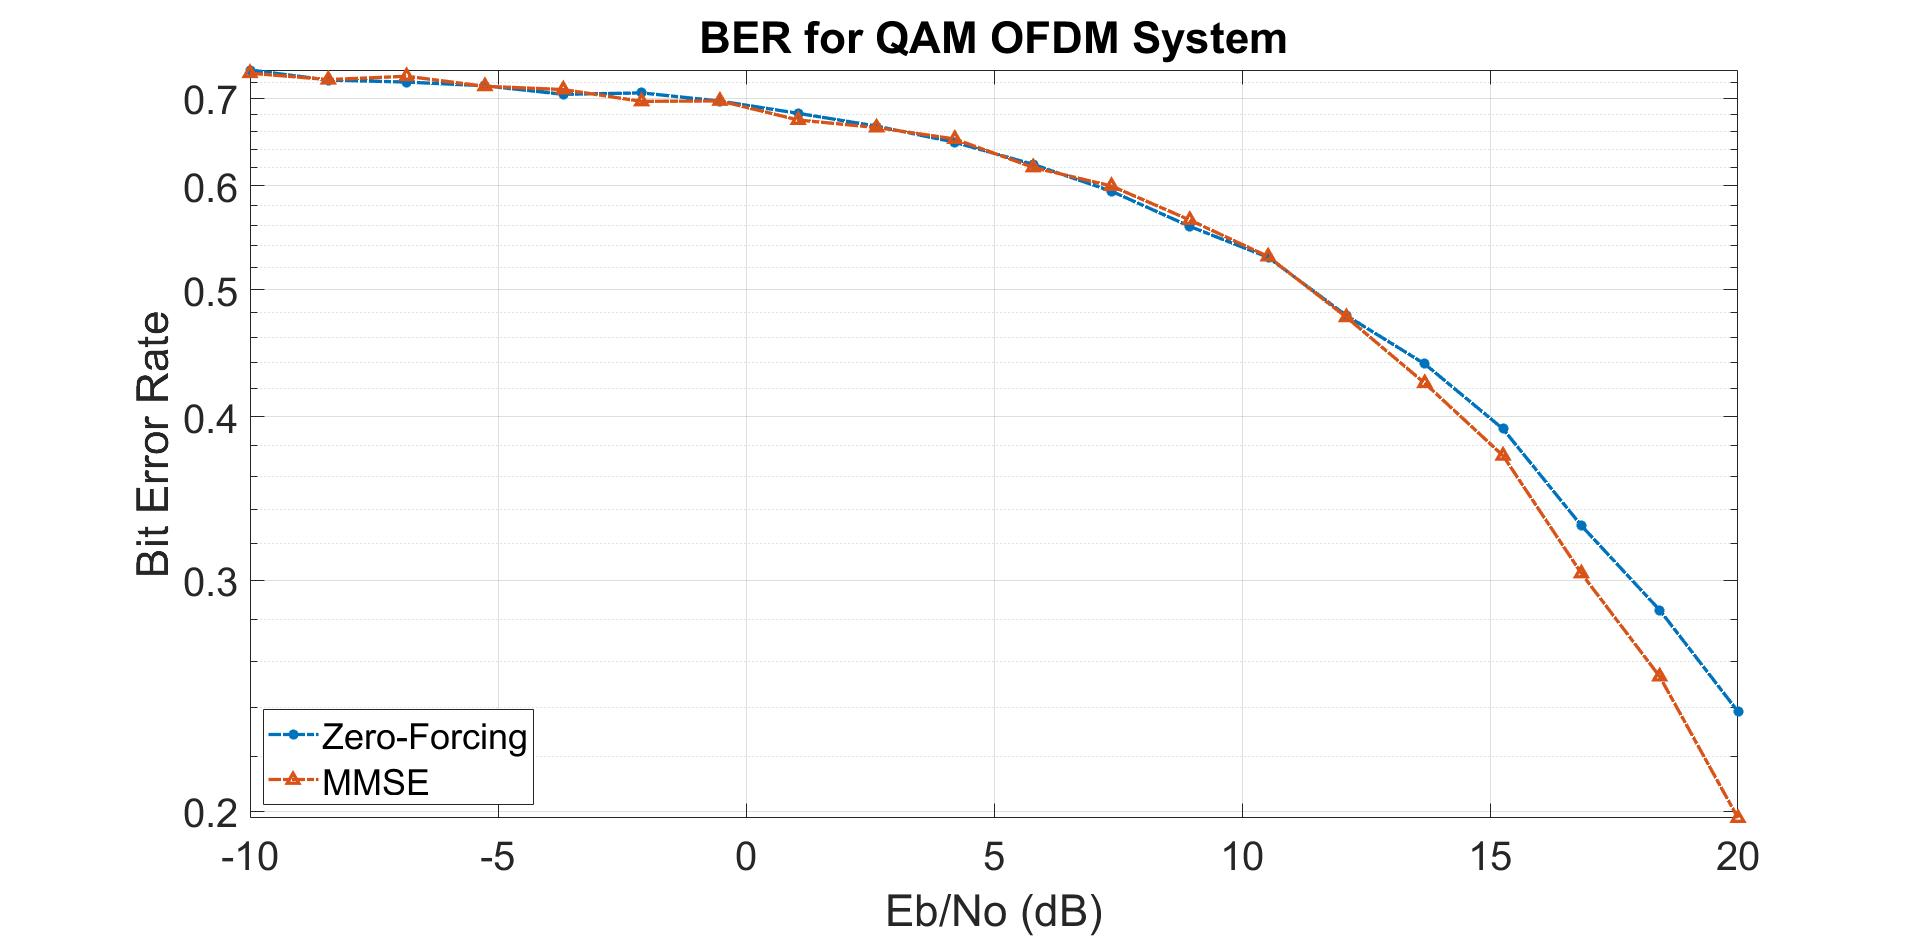
\includegraphics[width = 0.45\textwidth]{OFDM.jpg}
    \caption{BER plot for a QAM OFDM system using different OFDM algorithms.}
    \label{fig:ofdm_res}
\end{figure}

\section{MIMO-OFDM} \label{sec:MIMO-OFDM}
Finally, the two above systems were combined into six different systems, determined by one MIMO technique and one OFDM technique. They were similarly simulated over Gaussian random flat-fading channels and Rayleigh channels with AWGN noise. The results of this are shown in Fig.~\ref{fig:mimoofdm_res}.
\begin{figure}[!htbp]
    \centering
    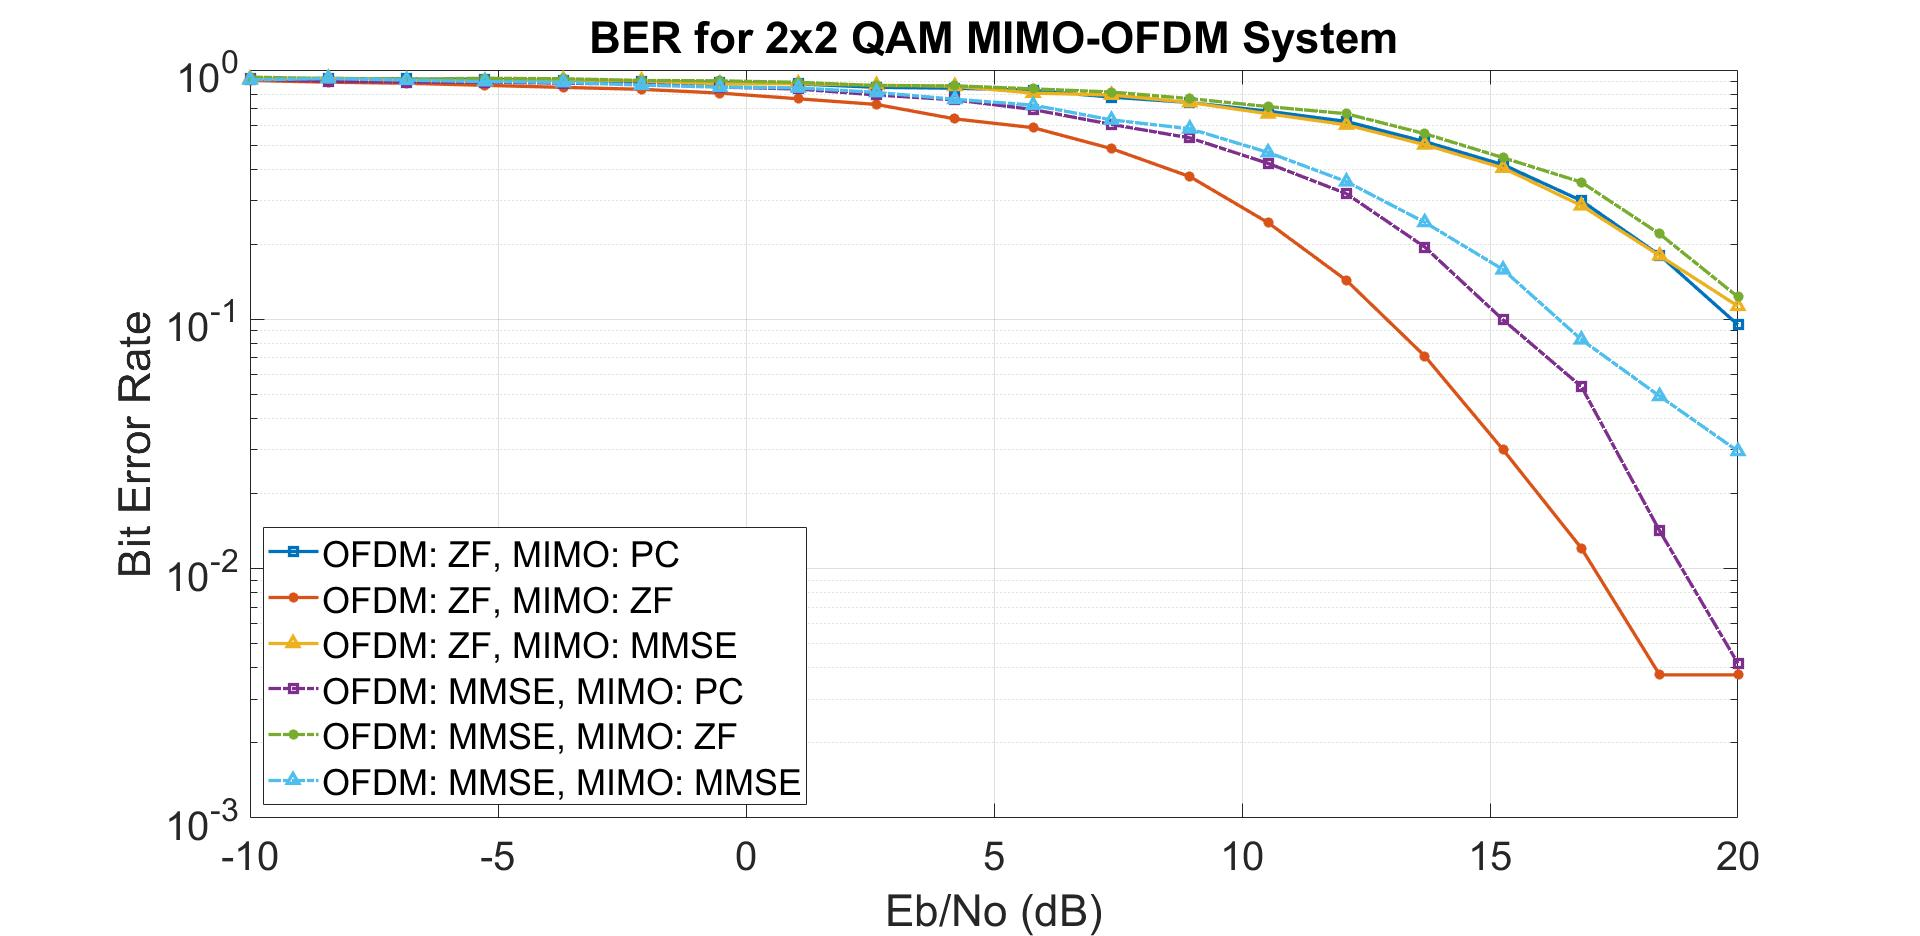
\includegraphics[width = 0.45\textwidth]{MIMOOFDM.jpg}
    \caption{BER plot for a $2\times2$ QAM hybrid MIMO-OFDM system using all combinations of the previous MIMO and OFDM algorithms.}
    \label{fig:mimoofdm_res}
\end{figure}

\section{Conclusion} \label{sec:conc}
A hybrid MIMO-OFDM system was simulated, both in parts and in tandem. Multiple techniques were used for equalization, and the performances of these techniques were compared.

%%%%%%%%%%%%%%%%%%% Bibliography %%%%%%%%%%%%%%%%%%%
\bibliographystyle{unsrt}
%% To reload citations:
%% F6 --> F11 --> F6 --> F6 --> F7
\bibliography{Bibliography} %filename (no .bib)

\end{document}